% Dúvidas do formato Latex?
% http://www.docs.is.ed.ac.uk/skills/documents/3722/3722-2014.pdf

% Sugestões de leitura
% https://seer.imed.edu.br/index.php/revistasi/article/view/1639/1296

\documentclass[12pt]{article}
\usepackage{sbc-rsa}
\usepackage{graphicx,url}
\usepackage[brazil]{babel}   
%\usepackage[latin1]{inputenc}  
\usepackage[utf8]{inputenc}  
% UTF-8 encoding is recommended by ShareLaTex

\sloppy

\title{Implementação e Análise de Complexidade do Sistema de Criptografia de Chave Pública RSA}

\author{Felipe Nathan Welter\inst{1}, Vitor Emanuel Batista\inst{1} }

\address{Centro de Ciências Tecnológicas -- Universidade do Estado de Santa Catarina
  (UDESC)\\
  89.219-710 -- Joinville -- SC -- Brazil
  \email{\{felipenwelter,vitorebatista\}@gmail.com}
}

\begin{document} 
\maketitle
\begin{resumo} 

O RSA é um algoritmo de criptografia assimétrica amplamente utilizado que permite garantir o estabelecimento de comunicações seguras em ambientes abertos como a internet. O objetivo desse artigo é descrever conceitualmente o funcionamento do algotirmo RSA e alguns pontos de seu embasamento matemático, a implementação realizada e sua complexidade, com o foco especial na análise de performance dos processos de geração e de quebra de chave. Dentro dos resultados atingidos é possível identificar que a segurança de sistemas de criptografia está baseada primordialmente na garantia de que a fatoração de grandes chaves demanda um tempo relativamente alto, mesmo para grande capacidade computacional. Nota-se também que a utilização de testes probabilísticos como os de Fermat e Miller-Rabin, assim como heurísticas como Pollard-Rho, permitem que se tenha ganho de performance, mas sem comprometer a segurança do sistema de criptografia.
\newline
\newline
Palavras-chave: Criptografia, RSA, Pollard Rho, Fermat, Miller-Rabin.

\end{resumo}


\section{Introdução}

A criptografia costuma ser definida como a arte de escrever em cifra ou em código, de modo a permitir que somente quem conheça o código possa ler a mensagem \cite{marcacini:10}. Com o crescente uso de dispositivos conectados a internet, como computadores, smartphones, equipamentos industriais (IIOT) e domésticos (IOT), tornam-se cada vez mais presentes na vida diária. Desta forma, a necessidade da segurança eletrônica torna-se ainda mais crítica. A utilização eficaz de técnicas criptográficas está no núcleo de várias dessas estratégias de gerenciamento de riscos de roubo de informações. \cite{burnett:02}


O sistema de criptografia de chave pública RSA se baseia na diferença drástica entre a facilidade de encontrar números primos grandes e a dificuldade de fatorar o produto de dois números primos grandes \cite{cormen:02}. A patente do algoritmo RSA expirou em setembro de 2000, o que permite que qualquer pessoa possa criar implementações desse algoritmo e, assim, aumentar ainda mais a utilização do RSA \cite{burnett:02}.


Neste artigo serão apresentados brevemente os conceitos da criptografia, com ênfase na criptografia RSA. Para o seu entendimento foram detalhadas alguns procedimentos fundamentais para sua construção, como a geração de números primos grandes e o inverso modular, assim como o ataque por força bruta para a quebra das chaves.

O artigo está divido em seções, sendo que a primeira apresenta a criptografia, seguida da seção de metodologia de implementação, apresentando os procedimentos para obtenção da RSA e o ataque de força bruta, assim como os resultados dos testes, por fim a conclusão do trabalho.


\section{Criptografia} \label{sec:firstpage}

Quando há necessidade de se proteger informações sigilosas utiliza-se o processo de criptografia para codificá-las de forma que não possam ser facilmente interpretadas. A leitura das informações criptografadas precisa passar por um novo processo de conversão, que é descriptografia, para que se torne novamente legível.

Um tipo muito comum de criptografia é chamado de chave simétrica. Nessa abordagem, um algoritmo utiliza uma chave para codificar informações em algo que se parece com um conjunto aleatório. O algoritmo, então, se utiliza da mesma chave para recuperar os dados originais \cite{burnett:02}.

Um sistema de criptografia de chave pública pode ser usado para codificar mensagens enviadas entre dois participantes de uma comunicação, de forma que um intruso que escute as mensagens codificadas não possa decodificá-las. Um sistema de criptografia de chave pública também permite que um dos participantes acrescente uma "assinatura digital"\ impossível de forjar ao final de uma mensagem eletrônica. Tal assinatura é a versão eletrônica de uma assinatura manuscrita em um documento de papel. Ela pode ser conferida com facilidade por qualquer pessoa, não pode ser forjada por ninguém, e ainda perde sua validade se qualquer bit da mensagem for alterado. Portanto, ela fornece autenticação, tanto da identidade do signatário quanto do conteúdo da mensagem assinada \cite{cormen:02}.

No sistema de criptografia RSA um usuário cria e torna pública uma chave baseada em dois números primos grandes, os quais são mantidos em segredo, ao mesmo tempo que cria uma chave privada, também mantida em segredo. Qualquer pessoa pode usar a chave pública para codificar uma mensagem e enviá-la ao destinatário que, em posse da chave privada, consegue descriptografá-la facilmente.

Cormen (2002) descreve os procedimentos a seguir, exemplificados pelos autores:
\begin{enumerate}
    \item Selecionar dois números primos grandes $p$ e $q$, sendo $p \neq q$, tal como 19 e 31;
    \item Calcular $n$ pela equação $n=p*q$, por exemplo $n$ = 589;
    \item Calcular o totiente de Euler, dado por $\phi(n) = (p-1)*(q-1)$, nesse caso $\phi(n) = 540$;
    \item Selecionar um inteiro ímpar pequeno $e$, tal que seja primo relativo de $\phi(n)$, satisfazendo a condição $MDC(e,\phi(n)) = 1$, nesse exemplo $e = 59$;
    \item Calcular $d$ como o inverso multiplicativo de $e$, utilizando o Algoritmo de Euclides estendido, que nesse exemplo resultaria em $d = 119$;
    \item O par formado por $P = (e,n)$ compõe a chave pública do RSA  e o par formado por $S = (d,n)$ a chave privada.
\end{enumerate}

O tamanho da chave é o fator mais importante para garantia da segurança no processo de criptografia. A Infraestrutura de Chaves Públicas do Brasil – ICP-Brasil recomenda o uso do algoritmo RSA como padrão para geração de chaves criptográficas de, no mínimo, 2048 bits \cite{icp:09}. A segurança do criptossistema RSA é fortemente vinculada à fatoração de $n$, que pode revelar os valores de $p$ e $q$. É devido ao grande esforço que demanda realizar essa fatoração e quebra da chave que se entende que o sistema de criptografia RSA é seguro. \cite{goodrich:13}.

\section{Implementação}

Para implementação do projeto e construção dos processos de criptografia, descriptografia e quebra de chaves foram utilizados diferentes algoritmos com o intuito de avaliar as diferenças de performance de execução. Para realizar o teste de primalidade foi aplicado um processo de Força Bruta pela fatoração de números, assim como foram aplicados algoritmos baseados no Teorema de Fermat e de Miller-Rabin. Para o cálculo do inverso modular, utilizado para montagem da chave privada, foi utilizado o Algoritmo de Euclides Estendido. Todas as implementações foram realizadas em Python 3, disponível de forma \textit{open source} no Github (https://github.com/vitorebatista/rsa-article)





\subsection{Teste de Primalidade}

Seguindo a estrutura descrita anteriormente, o primeiro passo consiste na definição de dois números primos aleatórios $p$ e $q$, sendo necessário realizar um teste de primalidade para garantir o atendimento dessa condição. A primalidade de um número se conceitua como um número inteiro positivo que tenha apenas dois divisores exatos, 1 e ele próprio.

Uma forma de garantir o teste de primalidade se dá pela fatoração do número, o que por meio de força bruta indica a realização de sucessivos testes até que se encontre uma divisão exata. Esse teste, entretanto se torna muito lento quando se trata de inteiros grandes. Para essa aplicação foram considerados dois diferentes métodos para verificação de primalidade: Fermat e Miller-Rabin. Nos dois casos não se obtém com exatidão se um número é ou não primo, porém devido a baixa probabilidade de erro e ganho de performance pode-se dizer conceitualmente que o número seria primo.

\textbf{Fermat:} o teorema de Fermat descreve que se um número $p$ é primo e $a$ é um inteiro tal que 1 $\leq$ a $\leq$ (p-1), então $\ a^{(p-1)} \equiv 1 (mod p)$. Existem alguns números, entrentanto, para o qual o teorema não se aplica, mas a garantia da primalidade se sustenta no fato de que o teste é realizado em rodadas, e que quanto mais rodadas se estabeleça, maior a probabilidade de $n$ ser primo.

A implementação de \texttt{is\underline{ }prime\underline{ }fermat} 
tem complexidade $O(k\log{}n)$, sendo $k$ o número de rodadas e $n$ o valor de entrada, visto a complexidade da função $pow$ para exponenciação.

\textbf{Miller-Rabin:} entendido como um dos testes mais eficientes da atualidade, também se baseia na operação de exponenciação modular. 


Cormen (2009, p. 706) menciona que a complexidade do algoritmo Miller-Rabin, com $n$ sendo um número de $\beta$ bits, exige $O(s\beta)$ operações aritméticas e $O(s\beta^{3})$ operações de bits, pois não exige assintoticamente mais trabalho que $s$ operações modulares. Sua complexidade pode ser definida como $O(k\log{}n)$, sendo $k$ o número de rodadas e $n$ o valor de entrada.


\subsection{Algoritmo de Euclides}

Para garantir a escolha de um número $e$ primo relativo de $\phi(n)$, utilizado na chave pública, assim como para se encontrar o número $d$, inverso multiplicativo de $e$ no módulo $\phi(n)$, utilizou-se do algoritmo de Euclides, que realiza sucessivas divisões com o resto que encontram o máximo divisor comum.

O algoritmo \texttt{gcd} realiza o cálculo do máximo divisor comum e tem complexidade de tempo $O(\log{}n)$, sendo $n$ o maior número de entrada. Por sua vez, o algoritmo \texttt{xgcd} realiza as mesmas divisões sucessivas de forma recursiva, retornando também o inverso multiplicativo dos valores de entrada $a$ e $b$ de forma a atender a expressão linear $ax+by=mdc(a,b)$. Sua complexidade de tempo é representada também por $O(\log{}n)$.

\subsection{Criptografia}

A implementação do algoritmo de criptografia foi centralizada por meio de uma classe, de forma que o cálculo dos valores relacionados às chaves fosse mais acessível e didático. É possível configurar tanto o método de teste de primalidade (força bruta, Fermat ou Miller-Rabin) quando o tamanho dos bits a serem utilizados.

Após a geração dos valores $p$ e $q$ o método \texttt{generate-keypair} realiza o cálculo dos valores $n$ e $\phi(n)$, assim como a definição do valor $e$ e cálculo do $d$, utilizados nas chaves pública e privada, respectivamente.

A criptografia em si consiste no recebimento de uma mensagem e da chave pública $(e,n)$, aplicadas na fórmula $c = m^e mod n$  considerando o código da tabela ASCII de cada caracter individualmente, o que é posteriormente salvo em um arquivo texto para consulta.

A descriptografia, por sua vez, realiza o procedimento inverso pela leitura do arquivo com o texto criptografado e aplicação do valor de cada caracter na fórmula $m = c^d mod n$, obtendo o valor original.


Para análise do tempo de execução foram realizadas combinações de algoritmos, contemplando diferentes processos para execução do teste de primalidade. A metodologia para coleta de dados consistiu na execução do processo de criptografia por 10 vezes consecutivas, com a exclusão das medições de menor e de maior valor. A implementação foi configurada para utilizar tamanhos de palavras variadas, de 4 em 4 bits até 32 bits. A Tabela~\ref{tab:encryptTable} demonstra a diferença de tempo para geração das chaves utilizando os algoritmos de primalidade por força bruta,Miller-Rabin e Fermat.

\begin{table}[!htbp]
\centering
\caption{Tempo de geração das chaves (em segundos) \textit{x} Número de Bits.}
\label{tab:encryptTable}
\begin{tabular}{|l|l|l|l|}
\hline
\textbf{Bits} & \textbf{Prime} & \textbf{Miller} & \textbf{Fermat} \\ \hline
\textbf{4} & 0.1035 & 0.0002 & 0.0005 \\ \hline
\textbf{8} & 0.2942 & 0.0002 & 0.0005 \\ \hline
\textbf{16} & 1.0023 & 0.0007 & 0.0007 \\ \hline
\textbf{24} & 6.9885 & 0.0004 & 0.0022 \\ \hline
\textbf{32} & 824.30 & 0.0013 & 0.0045 \\ \hline
\end{tabular}
\end{table}


É possível notar uma grande diferença de tempo entre o modelo de força bruta e a aplicação dos algoritmos Miller-Rabin e Fermat, o que se torna ainda mais evidente quando se aumenta o tamanho da chave. A melhor performance resultante dos testes foi do Algoritmo de Miller-Rabin, o que justifica ser o teste mais utilizado nas soluções de criptografia e um dos mais eficientes da atualidade \cite{ribeiro:2014}. No gráfico a seguir é possível visualizar as linhas que representam a complexidade de tempo exponencial para o algoritmo de força bruta (prime), em relação com o crescimento logarítmico dos algoritmos Miller-Rabin e Fermat. % (Dietzfelbinger 2004)

\begin{figure}[!htbp]
\centering
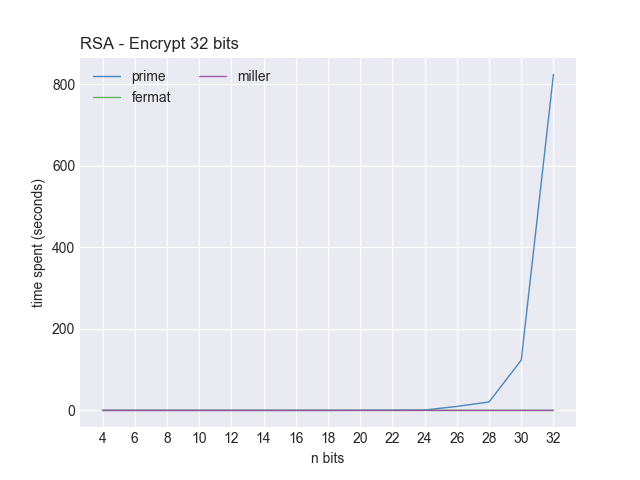
\includegraphics[width=0.75\textwidth]{images/32_Encrypt.png}
\caption{Tempo de geração das chaves (em segundos) \textit{x} Número de Bits.}
\label{fig:encryptFig}
\end{figure}


\subsection{Força bruta}


Um algoritmo de força bruta consiste na verificação sistemática de todas as possibilidades até que se consiga encontrar a correta para atender determinada condição. No pior caso o algoritmo precisaria percorrer todo o espaço de busca, o que demandaria um grande esforço computacional.

A força bruta para quebra da chave de criptografia consiste basicamente em conhecer o valor $n$ da chave pública e buscar $p$ e $q$ através de sucessivas divisões até que se encontre a operação que resulte em resto 0. Em posse de $p$ e $q$, calcula-se o totiente $\phi(n)$, e em seguida o inverso multiplicativo (via algoritmo de Euclides) para $\phi$ e $e$ da chave pública, encontrando $d$ da chave privada. Dependendo do tamanho da palavra, a busca por $p$ e $q$ pode demandar muito tempo, sendo essa a condição que garante a segurança do RSA.

Para realizar a quebra da chave também é possível se utilizar do algoritmo Pollard-Rho, que possui uma melhor performance nos casos em que a fatoração de grandes números que tenham fatores primos pequenos. A heurística se baseia em um algoritmo de detecção de ciclos para encontrar um dos valores gerados. Mesmo não garantindo tempo de execução, o pior cenário costuma ter complexidade $O(\sqrt{n})$, sendo $n$ o fator modular de $p$ e $q$ \cite{cormen:02}.

Na tabela~\ref{tab:breakTable} abaixo foi realizado um teste comparativo para averiguar a diferença de performance na quebra da chave utilizando de um algoritmo de força bruta (até $\sqrt{n}$) e Pollard-Rho. Para a geração de chave foram utilizados os mesmos algoritmos citados anteriormente e a comparação realizada contemplou todas as combinações de geração (Prime, Miller-Rabin e Fermat) e quebra de chave (Brutal Force e Pollard Rho).

% Please add the following required packages to your document preamble:
% \usepackage{multirow}
\begin{table}[!htbp]
\centering
\caption{Tempo de quebra de chaves (segundos) \textit{x} número de bits.}
\label{tab:breakTable}
\begin{tabular}{|c|l|l|l|l|l|l|}
\hline
\multirow{\textbf{Bits}} & \multicolumn{3}{c|}{\textbf{Brutal Force}} & \multicolumn{3}{c|}{\textbf{Pollard Rho}} \\ \cline{2-7} 
 & \textbf{Prime} & \textbf{Miller} & \textbf{Fermat} & \textbf{Prime} & \textbf{Miller} & \textbf{Fermat} \\ \hline
\textbf{4} & 0.0003 & 0.0002 & 0.0004 & 0.0002 & 0.0002 & 0.0002 \\ \hline
\textbf{8} & 0.0003 & 0.0003 & 0.0005 & 0.0003 & 0.0003 & 0.0003 \\ \hline
\textbf{16} & 0.0075 & 0.0062 & 0.0121 & 0.0061 & 0.0045 & 0.0038 \\ \hline
\textbf{24} & 1.3865 & 1.4948 & 1.4153 & 0.0576 & 0.0638 & 0.0803 \\ \hline
\textbf{32} & 621.03 & 476.90 & 667.88 & 1.1744 & 1.1017 & 1.3571 \\ \hline
\end{tabular}
\end{table}

A Figura~\ref{Fig:bruteforceFig} demonstra os tempos de quebra de chaves \textit{x} número de bits da chave para a implementação do ataque de força bruta proposto neste trabalho, assim como na Figura~\ref{Fig:pollardFig} a quebra de chaves com o algoritmo de \textit{Pollard Rho}. Analisando o gráfico percebe-se que o tempo de execução da função de quebra por força bruta é de complexidade de tempo exponencial em relação à quantidade de bits da entrada, tornando-se computacionalmente inviável a quebra de chaves com valores muito grandes. Contudo, é nítida a diferença de tempo de quebra de chaves via força bruta e Pollard Rho, valendo ressaltar a diferença na escala de tempo dos dois gráficos - Força Bruta de 0 a 600 segundos e Pollard Rho de 0 a 1.4 segundos.

\begin{figure}[!htbp]
   \begin{minipage}{0.48\textwidth}
     \centering
     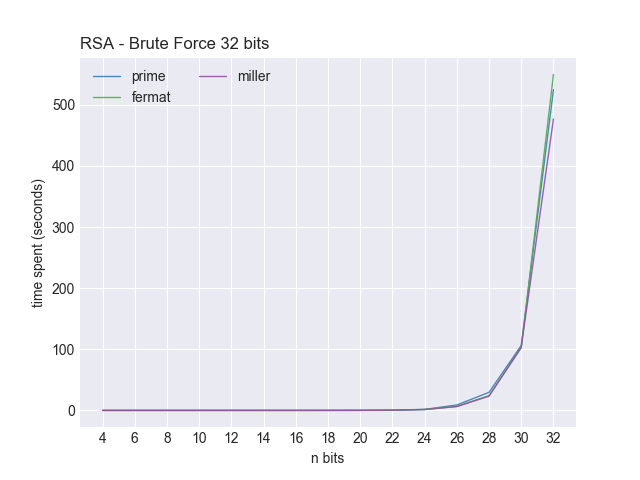
\includegraphics[width=1.1\linewidth]{images/32_BruteForce.png}
     \caption{Força bruta.}\label{Fig:bruteforceFig}
   \end{minipage}\hfill
   \begin{minipage}{0.48\textwidth}
     \centering
     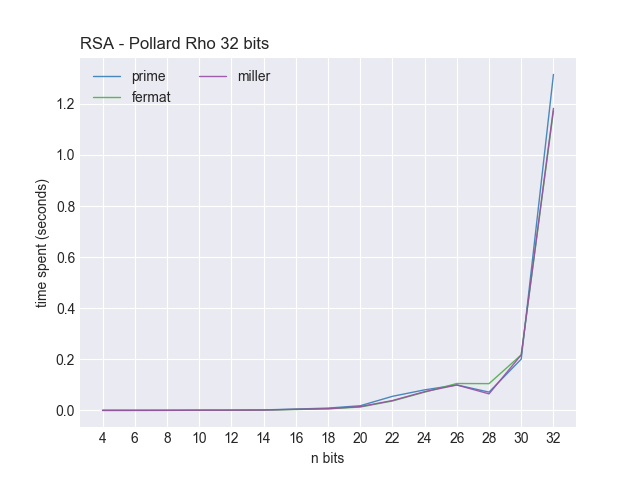
\includegraphics[width=1.1\linewidth]{images/32_PollardRho.png}
     \caption{Pollard Rho.}\label{Fig:pollardFig}
   \end{minipage}
\end{figure}



\section{Conclusão}

De modo algum a criptografia é a única ferramenta necessária para assegurar a segurança dos dados, nem resolverá todos os problemas de segurança. É um instrumento entre vários outros. Além disso, a criptografia não é à prova de falhas. Toda criptografia pode ser quebrada e, sobretudo, se for implementada incorretamente, ela não agrega nenhuma segurança real \cite{burnett:02}.



\bibliographystyle{sbc}
\bibliography{sbc-rsa}

\end{document}
